\begin{center}
\bfseries{\large ТЕХНИЧЕСКИЙ ОТЧЁТ ПО ПРАКТИКЕ}
\end{center}

\section*{Архитектура}

Архитектура проекта поддерживается самим движком Unity и инкапсулированна в нём. Каждый объект состоит из компонентов. Базовыми являются: координаты, коллайдеры, mesh-свойства, физические компоненты и т.д. Пользователь может писать собственные скрипты и прикреплять их в качестве новых компонент, а также редактировать свойства своих и базовых компонент.

\section*{Описание}

Взаимодействие с пользователем осуществляется через устройства ввода (клавиатуру и мышь). Пользователь может управлять положением камеры, закрепленной за протагонистом, а также его положением в пространстве. 
Игрок может взаимодействовать с объектами игрового мира. За такое взаимодействие отвечают скрипты, написанные на языке C\#. Данные скрипты обрабатывают ввод данных с клавиатуры и мыши, после чего просчитывается физические взаимодействия с объектами игрового мира.

\section*{Реализация}

\noindent {\bf SPlayerMoving.cs} Движение игрока

\begin{lstlisting}[language=csh]
using System.Collections;
using System.Collections.Generic;
using UnityEngine;

public class SPlayerMoving : MonoBehaviour
{
    public Transform target_rotation;

    public float player_speed = 0.7f;
    public float jump_size = 0.5f;
    public float max_jump_height = 2.0f;
    public float rotation_speed = 0.1f;

    private Rigidbody _player_rigidbody;

    void Start()
    {
        _player_rigidbody = GetComponent<Rigidbody>();

    }

    private Vector3 ProjectionOnXZ(Vector3 vector)
    {
        vector.y = 0f;
        return vector.normalized;
    }

    void FixedUpdate()
    {
        float horizontal = Input.GetAxisRaw("Horizontal");
        float vertical = Input.GetAxisRaw("Vertical");

        Vector3 move_vector = new Vector3(vertical, 0.0f, -horizontal).normalized;

        if (move_vector.magnitude > 0.1f)
        {
            _player_rigidbody.MoveRotation(Quaternion.Slerp(transform.rotation, Quaternion.LookRotation(ProjectionOnXZ(target_rotation.right)), rotation_speed));
        }
        _player_rigidbody.AddForce(((transform.right * -vertical) + (transform.forward * (horizontal))) * player_speed, ForceMode.VelocityChange);

        if (Input.GetKey(KeyCode.Space) && _player_rigidbody.position.y < max_jump_height)
        {
            _player_rigidbody.AddForce(Vector3.up * jump_size, ForceMode.VelocityChange);
        }
    }
}
\end{lstlisting}

\noindent {\bf SProCamera.cs}  Движение камеры за игроком

\begin{lstlisting}[language=csh]
using System.Collections;
using System.Collections.Generic;
using UnityEngine;

public class SProCamera : MonoBehaviour
{
    public Transform target;
    public float speedX = 300.0f;
    public float speedY = 400.0f;
    public float limitY = 90.0f;
    public float length_camera_react = 100.0f;
    public float length_player_react = 10.0f;
    public float min_obst_dist = 1.8f;
    public bool true_move;

    public LayerMask active;
    public LayerMask obstacles;
    public LayerMask no_player;

    private float _min_distance = 2.0f;
    private float _max_distance;
    private Vector3 _local_posotion;
    private float _current_y_rotation;
    public LayerMask _origin_mask;

    private GameObject _prev_select_obj;

    private Vector3 _position
    {
        get { return transform.position; }
        set { transform.position = value; }
    }

    void Start()
    {
        true_move = true;
        _prev_select_obj = null;
        _local_posotion = target.InverseTransformPoint(_position);
        _max_distance = Vector3.Distance(_position, target.position);
        _origin_mask = GetComponent<Camera>().cullingMask;
    }

    private void Update()
    {
        CameraReact();
    }

    private void LateUpdate()
    {
        _position = target.TransformPoint(_local_posotion);
        CameraRot();
        if (true_move)
        {
            CameraObst();
            CameraMinObstDist();
        } 
        _local_posotion = target.InverseTransformPoint(_position);
    }

    void CameraRot()
    {
        float move_x = Input.GetAxis("Mouse X");
        float move_y = -Input.GetAxis("Mouse Y");

        if (move_y != 0)
        {
            float tmp = Mathf.Clamp(_current_y_rotation + move_y * speedY * Time.deltaTime, -limitY, limitY);
            if (tmp != _current_y_rotation)
            {
                float r = tmp - _current_y_rotation;
                transform.RotateAround(target.position, transform.right, r);
                _current_y_rotation = tmp;
            }
        }

        if (move_x != 0)
        {
            transform.RotateAround(target.position, transform.up, move_x * speedX * Time.deltaTime);
        }

        transform.LookAt(target);
    }

    void CameraObst()
    {
        float distance = Vector3.Distance(_position, target.position);
        RaycastHit hit;

        if (Physics.Raycast(target.position, transform.position - target.position, out hit, _max_distance - _min_distance, obstacles))
        {
            _position = hit.point;
        } else if (distance < _max_distance && !Physics.Raycast(_position, -transform.forward, 0.1f, obstacles))
        {
            _position -= transform.forward * 0.05f;
        }
    }

    void CameraMinObstDist()
    {
        if (Vector3.Distance(_position, target.position) < min_obst_dist)
        {
            GetComponent<Camera>().cullingMask = no_player;
        } else
        {
            GetComponent<Camera>().cullingMask = _origin_mask;
        }
    }

    void CameraReact()
    {
        Ray ray_forward = new Ray(transform.position, transform.forward.normalized);
        RaycastHit hit;

        if (Physics.Raycast(ray_forward, out hit, length_camera_react, active) && (XZ(target.position) - XZ(hit.point)).magnitude < length_player_react)
        {

            GameObject obj = hit.collider.gameObject;

            if (_prev_select_obj && _prev_select_obj != obj)
            {
                if (_prev_select_obj.GetComponent<SSelect>() && _prev_select_obj.GetComponent<SSelect>().true_select)
                {
                    _prev_select_obj.GetComponent<SSelect>().Deselect();
                    _prev_select_obj = null;
                }
            }

            if (obj.GetComponent<SSelect>())
            {
                _prev_select_obj = obj;
                obj.GetComponent<SSelect>().Select();
            }
        }
        else if (_prev_select_obj && _prev_select_obj.GetComponent<SSelect>() && _prev_select_obj.GetComponent<SSelect>().true_select)
        {
            _prev_select_obj.GetComponent<SSelect>().Deselect();
            _prev_select_obj = null;
        }

    }

    Vector3 XZ(Vector3 vector)
    {
        vector.y = 0;
        return vector;
    }
}
\end{lstlisting}

\noindent {\bf SGun.cs} Стрельба из оружия

\begin{lstlisting}[language=csh]
using System.Collections;
using System.Collections.Generic;
using UnityEngine;

public class SGun : MonoBehaviour
{
    public GameObject bullet;
    // Start is called before the first frame update
    void Start()
    {
        
    }

    // Update is called once per frame
    void Update()
    {
        if (Input.GetKeyDown(KeyCode.F))
        {
            GameObject new_bull = Instantiate(bullet, transform.position + new Vector3(0.5f, 0.1f, 0.0f), transform.rotation);
            new_bull.GetComponent<Rigidbody>().velocity = -new_bull.transform.right * 30.0f;
        }

    }
}
\end{lstlisting}

\noindent {\bf SBullet.cs} Взаимодействие пули с врагами

\begin{lstlisting}[language=csh]
using System.Collections;
using System.Collections.Generic;
using UnityEngine;

public class SBullet : MonoBehaviour
{

    private void OnCollisionEnter(Collision target)
    {
        if (target.gameObject.tag == "GunTarget")
        {
            Destroy(target.gameObject);
        }
    }
}

\end{lstlisting}

\noindent {\bf SCapRotation.cs} Вращение шляпки

\begin{lstlisting}[language=csh]
using System.Collections;
using System.Collections.Generic;
using UnityEngine;

public class SCapRotation : MonoBehaviour
{
    public float cap_speed = 2.0f;

    private Transform _player_transform;
    // Start is called before the first frame update
    void Start()
    {
        _player_transform = transform.parent;
    }

    // Update is called once per frame
    void Update()
    {
        transform.RotateAround(_player_transform.position, transform.up, cap_speed);
    }
}
\end{lstlisting}

\noindent {\bf STargetForCamera.cs} Перемещение цели для камеры за игроком

\begin{lstlisting}[language=csh]
using System.Collections;
using System.Collections.Generic;
using UnityEngine;

public class STargetForCamera : MonoBehaviour
{
    public Transform player;

    private Vector3 _local_posotion;
    // Start is called before the first frame update
    void Start()
    {
        _local_posotion = player.InverseTransformPoint(transform.position);
    }

    // Update is called once per frame
    void Update()
    {
        transform.position = player.TransformPoint(_local_posotion);
        _local_posotion = player.InverseTransformPoint(transform.position);
    }
}
\end{lstlisting}

\noindent {\bf SStartGame.cs} Старт игры и переключение сцены

\begin{lstlisting}[language=csh]
using System.Collections;
using System.Collections.Generic;
using UnityEngine;
using UnityEngine.SceneManagement;

public class SStartGame : MonoBehaviour
{
    public void PlayPressed()
    {
        Cursor.lockState = CursorLockMode.Locked;
        Cursor.visible = false;
        SceneManager.LoadScene("Game");
    }

    public void ExitPressed()
    {
        Application.Quit();
    }
}
\end{lstlisting}

\noindent {\bf SSelect.cs} Триггер объекта на приблежение игрока

\begin{lstlisting}[language=csh]
using System.Collections;
using System.Collections.Generic;
using UnityEngine;

public class SSelect : MonoBehaviour
{
    public bool true_select;

    public void Start()
    {
        true_select = false;
    }

    public void Select()
    {
        true_select = true;
    }

    public void Deselect()
    {
        true_select = false;
    }
}
\end{lstlisting}

\noindent {\bf SOpenDoor.cs} Открывание двери

\begin{lstlisting}[language=csh]
using System.Collections;
using System.Collections.Generic;
using UnityEngine;

public class SOpenDoor : MonoBehaviour
{
    public float speed_open = 1.0f;
    public bool is_open;
    public Transform panel;
    public Transform door;

    //private BoxCollider _box_door;
    private Quaternion _close_rotation;
    private Quaternion _open_rotation;

    private SSelect _select;

    private Color _panal_color;

    //Start is called before the first frame update
    void Start()
    {
        _select = GetComponent<SSelect>();
        _panal_color = panel.GetComponent<Renderer>().material.color;

        _close_rotation = door.rotation;
        _open_rotation = Quaternion.LookRotation(-door.transform.right);
        is_open = false;

    }

    // Update is called once per frame
    void Update()
    {
        if (_select.true_select)
        {
            if (Input.GetKeyDown(KeyCode.E))
            {
                is_open = !is_open;
            }
            else
            {
                if (is_open) panel.GetComponent<Renderer>().material.color = Color.green;
                if (!is_open) panel.GetComponent<Renderer>().material.color = Color.magenta;
            }

        }
        else
        {
            panel.GetComponent<Renderer>().material.color = _panal_color;
        }

    }

    private void LateUpdate()
    {
        Rotate();
    }

    void Rotate()
    {
        if (door.rotation != _open_rotation && is_open)
            door.rotation = Quaternion.RotateTowards(door.rotation, _open_rotation, speed_open);

        if (door.rotation != _close_rotation && !is_open)
            door.rotation = Quaternion.RotateTowards(door.rotation, _close_rotation, speed_open);
    }


}
\end{lstlisting}

\noindent {\bf SEnterCodeCanvas.cs} Ввод кода в панель

\begin{lstlisting}[language=csh]
using System.Collections;
using System.Collections.Generic;
using UnityEngine;
using UnityEngine.UI;

public class SEnterCodeCanvas : MonoBehaviour
{
    [SerializeField]
    private Text _panel;
    public bool _entering;

    public void Start()
    {
        _entering = true;
    }
    public void Enter1(string text)
    {
        if (_entering)
        {
            _panel.text += text;
        }
    }
}
\end{lstlisting}

\noindent {\bf SEnterCode.cs} Механика ввода кода

\begin{lstlisting}[language=csh]
using System.Collections;
using System.Collections.Generic;
using UnityEngine;

public class SEnterCode : MonoBehaviour
{
    [SerializeField]
    private GameObject _note;
    private Camera _camera;
    private SSelect _select;
    private bool _is_active;
    private float[] _speedXandY;

    private Material _note_material;

    void Start()
    {
        _select = GetComponent<SSelect>();
        _note.SetActive(false);
        _is_active = false;
        _note_material = GetComponent<Renderer>().material;
        _camera = Camera.main;
        _speedXandY = new float[2] { _camera.GetComponent<SProCamera>().speedX, _camera.GetComponent<SProCamera>().speedY };
    }

    void Update()
    {
        if (_select.true_select)
        {
            _note_material.EnableKeyword("_EMISSION");

            if (Input.GetKeyDown(KeyCode.E) && !_is_active)
            {
                Activate();
            }

            if (Input.GetKeyDown(KeyCode.Q) && _is_active)
            {
                Deactivate();
                Cursor.lockState = CursorLockMode.Locked;
                Cursor.visible = false;
            }

        }
        else
        {
            if (_is_active)
            {
                Cursor.lockState = CursorLockMode.Locked;
                Cursor.visible = false;
            }
            _note_material.DisableKeyword("_EMISSION");
            Deactivate();
        }
    }

    void Activate()
    {
        Cursor.lockState = CursorLockMode.Confined;
        Cursor.visible = true;
        _camera.GetComponent<SProCamera>().speedX = 0f;
        _camera.GetComponent<SProCamera>().speedY = 0f;

        _note.SetActive(true);
        _is_active = true;
    }

    void Deactivate()
    {
        _camera.GetComponent<SProCamera>().speedX = _speedXandY[0];
        _camera.GetComponent<SProCamera>().speedY = _speedXandY[1];

        _note.SetActive(false);
        _is_active = false;
    }
}
\end{lstlisting}

\noindent {\bf SCodeConfirm.cs} Подтверждение ввода кода

\begin{lstlisting}[language=csh]
using System.Collections;
using System.Collections.Generic;
using UnityEngine;
using UnityEngine.UI;

public class SCodeConfirm : MonoBehaviour
{
    [SerializeField]
    private string _confirmed_text;
    [SerializeField]
    private GameObject _object_to_action;
    [SerializeField]
    private SEnterCodeCanvas _sEnterCodeCanvas_entering;
    private SOpenDoor _action;
    private Text _text;

    void Start()
    {
        _text = GetComponent<Text>();
        _action = _object_to_action.GetComponent<SOpenDoor>();
    }

    void Update()
    {
        if (_text.text == _confirmed_text)
        {
            _action.speed_open = 1.5f;
            _sEnterCodeCanvas_entering._entering = false;
            _text.text = _confirmed_text;
            _text.color = Color.green;
        }
        else if (_text.text.Length >= 4)
        {
            _text.text = "";
        }
    }
}
\end{lstlisting}

\noindent {\bf SReadNote.cs} Чтение записки

\begin{lstlisting}[language=csh]
using System.Collections;
using System.Collections.Generic;
using UnityEngine;

public class SReadNote : MonoBehaviour
{
    [SerializeField] 
    private GameObject _note;
    private SSelect _select;
    private bool _is_active;

    private Material _note_material;

    void Start()
    {
        _select = GetComponent<SSelect>();
        _note.SetActive(false);
        _is_active = false;
        _note_material = GetComponent<Renderer>().material;
    }

    void Update()
    {
        if (_select.true_select)
        {
            _note_material.EnableKeyword("_EMISSION");

            if (Input.GetKeyDown(KeyCode.E) && !_is_active)
            {
                Activate();
            }
            
            if (Input.GetKeyDown(KeyCode.Q) && _is_active)
            {
                Deactivate();
            }

        } else
        {
            _note_material.DisableKeyword("_EMISSION");
            Deactivate();
        }
    }

    void Activate()
    {
        _note.SetActive(true);
        _is_active = true;
    }

    void Deactivate()
    {
        _note.SetActive(false);
        _is_active = false;
    }
}
\end{lstlisting}

\noindent {\bf SNumber.cs} Взаимодествие цифр из игры "пятнашки" друг с другом

\begin{lstlisting}[language=csh]
using System.Collections;
using System.Collections.Generic;
using UnityEngine;

public class SNumber : MonoBehaviour
{
    public Transform numbers;
    public LayerMask active;
    public Vector3 true_position;
    public bool act;
    public bool ok;

    private SSelect _select;
    private BoxCollider _box;
    private Color _origin_color;
    private float _min_distance;
    private Vector3 _move_x;
    private Vector3 _move_y;

    private Vector3 _1_position,  _2_position, _3_position;
    private Vector3 _4_position,  _5_position,  _6_position;
    private Vector3 _7_position,  _8_position;

    // Start is called before the first frame update
    void Start()
    {
        act = false; ok = false;
        _select = GetComponent<SSelect>();
        _box = GetComponent<BoxCollider>();

        true_position = new Vector3(transform.position.x, transform.position.y, transform.position.z);

        _1_position = numbers.Find("1").transform.position; _2_position = numbers.Find("2").transform.position;
        _3_position = numbers.Find("3").transform.position; _4_position = numbers.Find("4").transform.position;
        _5_position = numbers.Find("5").transform.position; _6_position = numbers.Find("6").transform.position;
        _7_position = numbers.Find("7").transform.position; _8_position = numbers.Find("8").transform.position;

        _origin_color = Color.HSVToRGB(22.0f, 77.0f, 32.0f);
        GetComponent<Renderer>().material.color = Color.white;
        _move_x = _1_position - _2_position;
        _move_y = _4_position - _7_position;
        _min_distance = transform.right.normalized.magnitude;
    }

    // Update is called once per frame
    void Update()
    {
        if (!ok && _select.true_select && act)
        {
            GetComponent<Renderer>().material.color = Color.green;
            Moving();

        }

        if (!ok && !_select.true_select && act)
        {
            GetComponent<Renderer>().material.color = _origin_color;
        }

        if (!act)
        {
            GetComponent<Renderer>().material.color = Color.white;
            
        }
        if (ok)
        {
            GetComponent<Renderer>().material.color = Color.magenta;
        }
    }

    void LateUpdate()
    {
        if (!act)
            StartPosition();

    }

    void Moving()
    {
        Ray ray_right = new Ray(transform.position, transform.right.normalized);
        Ray ray_left = new Ray(transform.position, -transform.right.normalized);
        Ray ray_up = new Ray(transform.position, transform.up.normalized);
        Ray ray_down = new Ray(transform.position, -transform.up.normalized);

        Debug.DrawRay(ray_right.origin, ray_right.direction, Color.red);
        Debug.DrawRay(ray_left.origin, ray_left.direction, Color.blue);
        Debug.DrawRay(ray_up.origin, ray_up.direction, Color.green);
        Debug.DrawRay(ray_down.origin, ray_down.direction, Color.yellow);

        if (Input.GetMouseButtonDown(0))
        {
            bool true_hit_right = Physics.Raycast(ray_right, _min_distance, active);
            bool true_hit_left = Physics.Raycast(ray_left, _min_distance, active);
            bool true_hit_up = Physics.Raycast(ray_up, _min_distance, active);
            bool true_hit_down = Physics.Raycast(ray_down, _min_distance, active);

            if (!true_hit_right) transform.position += _move_x;
            else if (!true_hit_left) transform.position -= _move_x;
            else if (!true_hit_up) transform.position += _move_y;
            else if (!true_hit_down) transform.position -= _move_y;
        }
    }
    void StartPosition()
    {
        numbers.Find("1").transform.position = _1_position;
        numbers.Find("2").transform.position = _2_position + _right;
        numbers.Find("3").transform.position = _3_position + _down;
        numbers.Find("4").transform.position = _4_position;
        numbers.Find("5").transform.position = _5_position + _up;
        numbers.Find("6").transform.position = _6_position + _down;
        numbers.Find("7").transform.position = _7_position;
        numbers.Find("8").transform.position = _8_position + _up;
    }
    private void Check()
    {
        if (transform.position == true_position)
        {
            GetComponent<Renderer>().material.color = Color.magenta;
        }
    }

    private Vector3 _right
    {
        get { return -_move_x; }
    }

    private Vector3 _left
    {
        get { return _move_x; }
    }

    private Vector3 _down
    {
        get { return -_move_y; }
    }

    private Vector3 _up
    {
        get { return _move_y; }
    }
}
\end{lstlisting}

\noindent {\bf SPlayNumb.cs} Механика игры "пятнашки"

\begin{lstlisting}[language=csh]
using System.Collections;
using System.Collections.Generic;
using UnityEngine;

public class SPlayNumb : MonoBehaviour
{
    public Transform panel;
    public Transform numbers;
    public GameObject lamp;
    public bool active;
    public bool finish;

    private SSelect _select;
    private Color _origin_color;

    private SNumber _1, _2, _3;
    private SNumber _4, _5, _6;
    private SNumber _7, _8;

    // Start is called before the first frame update
    void Start()
    {
        _select = GetComponent<SSelect>();
        _1 = Pos("1"); _2 = Pos("2"); _3 = Pos("3");
        _4 = Pos("4"); _5 = Pos("5"); _6 = Pos("6");
        _7 = Pos("7"); _8 = Pos("8");

        _origin_color = panel.GetComponent<Renderer>().material.color;
        active = false;
        finish = false;
        if (lamp.GetComponent<Light>().enabled)
            lamp.GetComponent<Light>().enabled = false;
    }

    // Update is called once per frame
    void Update()
    {
        if (_select.true_select)
        {
            if (!active) panel.GetComponent<Renderer>().material.color = Color.green;
            if (Input.GetKeyDown(KeyCode.E))
                active = !active;
        } else
        {
            panel.GetComponent<Renderer>().material.color = _origin_color;
        }

        if (active)
            panel.GetComponent<Renderer>().material.color = Color.magenta;
        else if (!_select)
            panel.GetComponent<Renderer>().material.color = _origin_color;
        
    }

    private void LateUpdate()
    {
        if (active)
        {
            Activation();
            Check();
        }
        else
        {
            Deactivation();
        }
    }

    private void Activation()
    {
        _1.act = true; _2.act = true; _3.act = true;
        _4.act = true; _5.act = true; _6.act = true;
        _7.act = true; _8.act = true;
    }

    private void Deactivation()
    {
        _1.act = false; _2.act = false; _3.act = false;
        _4.act = false; _5.act = false; _6.act = false;
        _7.act = false; _8.act = false;
    }

   private void Check()
    {
        if (InTruePosition(_1) && InTruePosition(_2) &&
            InTruePosition(_3) && InTruePosition(_4) &&
            InTruePosition(_5) && InTruePosition(_6) &&
            InTruePosition(_7) && InTruePosition(_8))
        {
            _1.ok = true; _2.ok = true; _3.ok = true;
            _4.ok = true; _5.ok = true; _6.ok = true;
            _7.ok = true; _8.ok = true;

            if (!finish)
                lamp.GetComponent<Light>().enabled = true;
            finish = true;
        }

    }

    private SNumber Pos(string num)
    {
        return numbers.Find(num).GetComponent<SNumber>();
    }

    private bool InTruePosition(SNumber num)
    {
        return num.transform.position == num.true_position;
    }



}
\end{lstlisting}

\noindent {\bf SPlayLmp.cs} Игра со светом

\begin{lstlisting}[language=csh]
using System.Collections;
using System.Collections.Generic;
using UnityEngine;

public class SPlayLmp : MonoBehaviour
{
    public Transform lmp;
    public Transform light1;
    public GameObject light2;
    public GameObject light3;
    public GameObject first_lamp;
    public GameObject second_lamp;

    private SSelect _select;
    private Color _origin_color;
    private bool _end;
    // Start is called before the first frame update
    void Start()
    {
        _end = false;
        _select = GetComponent<SSelect>();
        _origin_color = GetComponent<Renderer>().material.color;

        if (first_lamp.GetComponent<Light>().enabled)
            first_lamp.GetComponent<Light>().enabled = false;

        if (second_lamp.GetComponent<Light>().enabled)
            second_lamp.GetComponent<Light>().enabled = false;

        if (light3.GetComponent<Light>().enabled)
            light3.GetComponent<Light>().enabled = false;
    }

    // Update is called once per frame
    void Update()
    {
        if (light2.GetComponent<Light>().enabled)
        {
            if (_select.true_select)
            {
                GetComponent<Renderer>().material.color = Color.grey;
                if (Input.GetKeyDown(KeyCode.E))
                {
                    GetComponent<Renderer>().material.color = Color.blue;
                    if (first_lamp.GetComponent<Light>().enabled)
                        first_lamp.GetComponent<Light>().enabled = false;
                    else first_lamp.GetComponent<Light>().enabled = true;

                    if (second_lamp.GetComponent<Light>().enabled)
                        second_lamp.GetComponent<Light>().enabled = false;
                    else second_lamp.GetComponent<Light>().enabled = true;
                }

            }
            else
            {
                GetComponent<Renderer>().material.color = _origin_color;
            }
            
        }
    }
    void LateUpdate()
    {
        Check();
        if (light2.GetComponent<Light>().enabled) Check();
    }

    void Check()
    {
        bool ok = true;
        foreach (Transform l in lmp.GetComponentInChildren<Transform>())
        {
            if (!l.GetComponent<Light>().enabled)
                ok = false;
        }
        if (ok && !_end)
        {
            if (light2.GetComponent<Light>().enabled)
                light2.GetComponent<Light>().enabled = false;

            if (!light3.GetComponent<Light>().enabled)
                light3.GetComponent<Light>().enabled = true;

            light1.RotateAround(light1.position, light1.right, 175.0f);
            light1.GetComponent<Light>().intensity = light1.GetComponent<Light>().intensity / 1.4f;
            _end = true;
        }
        

    }

}
\end{lstlisting}

\noindent {\bf SPlace.cs} Панель для игры в "пятнашки"

\begin{lstlisting}[language=csh]
using System.Collections;
using System.Collections.Generic;
using UnityEngine;

public class SPlace : MonoBehaviour
{
    public Camera cam;
    public Transform player;
    public GameObject panel_numb;

    private float _min_distanse = 0.5f;
    private float _origin_dist;
    private bool _act;

    private void Start()
    {
        _origin_dist = cam.GetComponent<SProCamera>().length_player_react;
        _act = true;
    }

    // Update is called once per frame
    void Update()
    {
        if (Vector3.Distance(player.position, transform.position) < _min_distanse && panel_numb.GetComponent<SPlayNumb>().active && _act)
        {
            cam.GetComponent<SProCamera>().true_move = false;
            cam.GetComponent<SProCamera>().length_player_react = 50;
            cam.GetComponent<Camera>().cullingMask = cam.GetComponent<SProCamera>().no_player;
        } else if (_act)
        {
            cam.GetComponent<Camera>().cullingMask = cam.GetComponent<SProCamera>()._origin_mask;
            cam.GetComponent<SProCamera>().length_player_react = _origin_dist;
            cam.GetComponent<SProCamera>().true_move = true;
        }

        if (panel_numb.GetComponent<SPlayNumb>().finish && _act)
        {
            cam.GetComponent<Camera>().cullingMask = cam.GetComponent<SProCamera>()._origin_mask;
            cam.GetComponent<SProCamera>().length_player_react = _origin_dist;
            cam.GetComponent<SProCamera>().true_move = true;
            _act = false;
        }
    }
}
\end{lstlisting}

\noindent {\bf SPanelKey.cs} Поучение игрового трофея - оружия

\begin{lstlisting}[language=csh]
using System.Collections;
using System.Collections.Generic;
using UnityEngine;

public class SPanelKey : MonoBehaviour
{
    public GameObject light3;
    public GameObject key;
    public Transform key_cube;
    public GameObject gun;
    public GameObject cap;

    private GameObject new_key;
    private bool _get_key;
    private SSelect _select;
    private Color _origin_color;
    private bool _ok;
    private Color _origin_color_key;
    private float _min_dist = 2.0f;

    // Start is called before the first frame update
    void Start() {
        _get_key = false;
        _origin_color = GetComponent<Renderer>().material.color;
        _select = GetComponent<SSelect>();
        _ok = true;
    }

    // Update is called once per frame
    void Update()
    {
        if (light3.GetComponent<Light>().enabled)
        {
            if (_select.true_select)
            {
            GetComponent<Renderer>().material.color = Color.green;

            if (Input.GetKeyDown(KeyCode.E)) GetKey();
            }
            else
            {
                GetComponent<Renderer>().material.color = _origin_color;
            }
        }

        if (_get_key && _ok)
        {
            if (Vector3.Distance(new_key.transform.position, cap.transform.position) < _min_dist)
            {
                new_key.GetComponent<Renderer>().material.color = Color.green;
                if (Input.GetKeyDown(KeyCode.E))
                {
                    PutOn();
                    _ok = false;
                }
            } else
            {
                new_key.GetComponent<Renderer>().material.color = _origin_color_key;
            }
        }

    }

    void GetKey()
    {
        if (!_get_key)
        {
            float pos_z = key_cube.GetComponents<Collider>().Length;
            new_key = Instantiate(key, key_cube.position + new Vector3(0.0f, 0.0f, -pos_z), key_cube.rotation);
            new_key.GetComponent<Rigidbody>().velocity = key_cube.right * 4.0f;
            _origin_color_key = new_key.GetComponent<Renderer>().material.color;
            _get_key = true;
        }
    }

    void PutOn()
    {
        if (new_key.activeSelf) new_key.SetActive(false);
        if (cap.activeSelf) cap.SetActive(false);
        if (!gun.activeSelf) gun.SetActive(true);
        
    }

}
\end{lstlisting}

\noindent {\bf SEnemy.cs} Движение врагов

\begin{lstlisting}[language=csh]
using System.Collections;
using System.Collections.Generic;
using UnityEngine;

public class SEnemy : MonoBehaviour
{
    public Transform start_point;
    public float enemy_speed = 0.3f;
    private Vector3 move_vect;
    // Start is called before the first frame update
    void Start()
    {
        move_vect = transform.forward;
    }

    // Update is called once per frame
    void Update()
    {
        transform.position += move_vect * enemy_speed;
    }

    private void OnCollisionEnter(Collision collision)
    {
        if (collision.gameObject.tag == "Obstacles")
        {
            if (move_vect == transform.forward)
                move_vect = -transform.forward;
            else
                move_vect = transform.forward;
        }

        if (collision.gameObject.tag == "Player")
        {
            collision.gameObject.transform.position = start_point.position;
        }
    }
}
\end{lstlisting}

\noindent {\bf 3D-модели:}

Модели объектов, созданные в Blender.

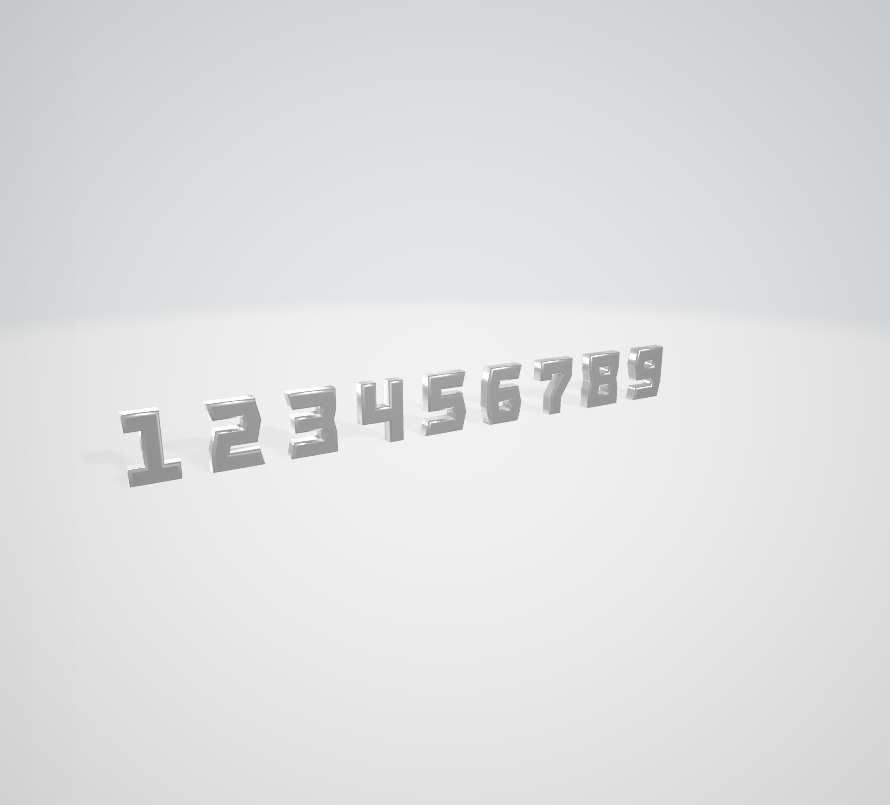
\includegraphics[scale=0.25]{images/1.jpg}
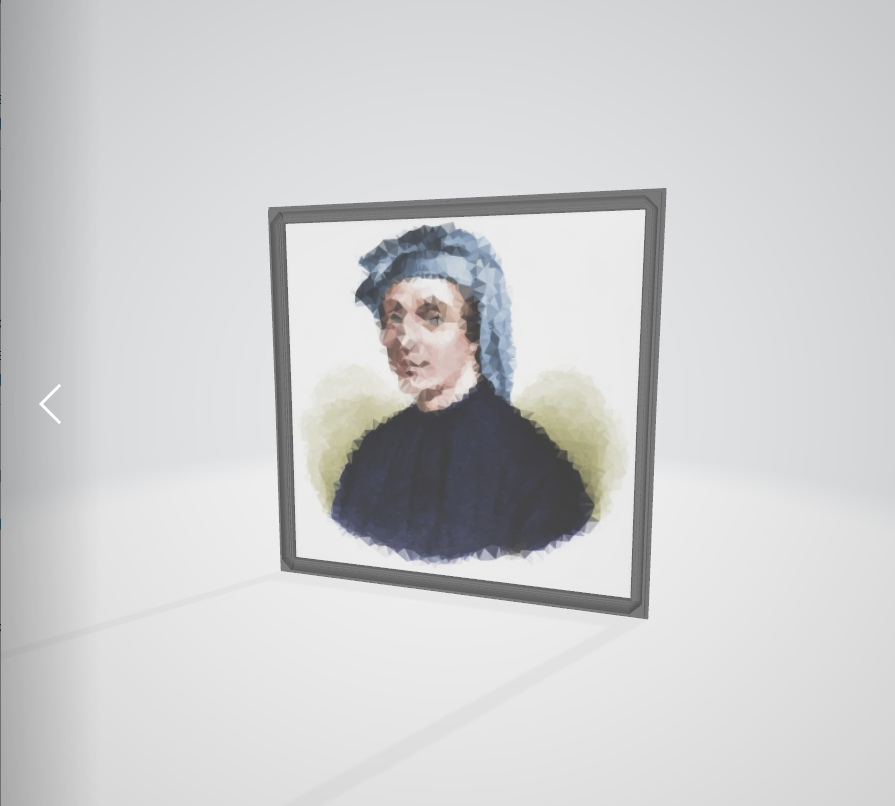
\includegraphics[scale=0.25]{images/2.jpg} \\
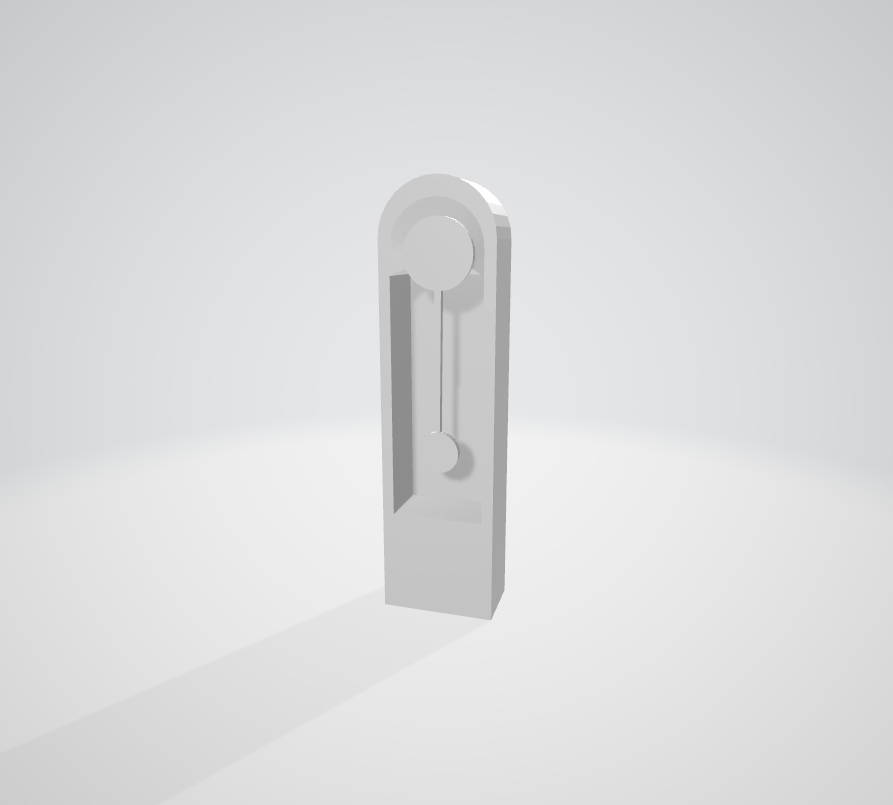
\includegraphics[scale=0.25]{images/3.jpg}
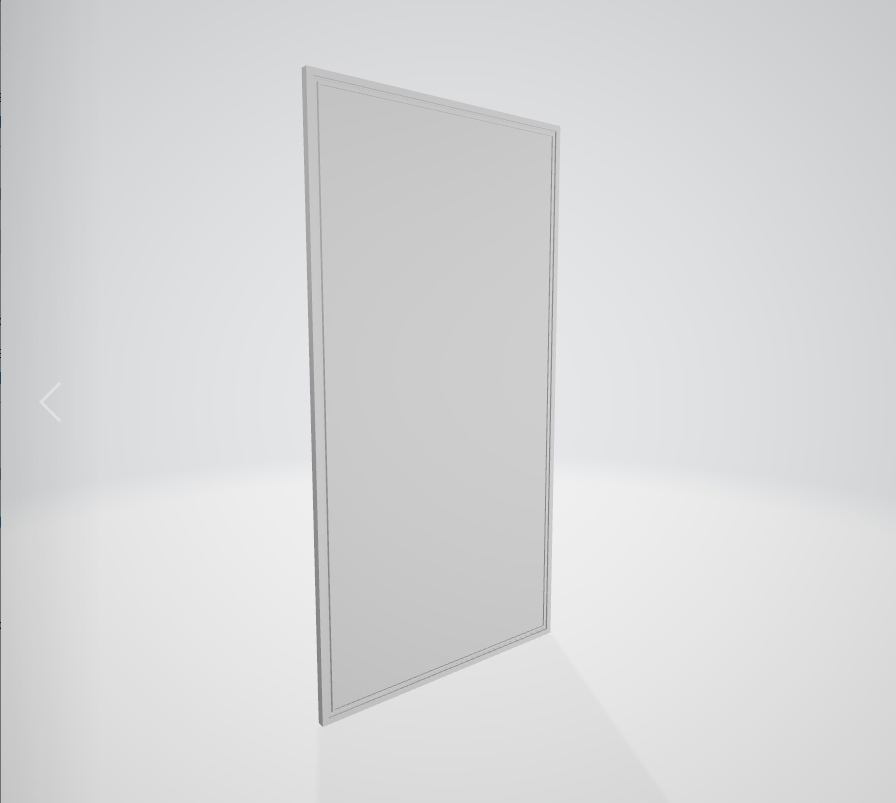
\includegraphics[scale=0.25]{images/4.jpg} \\
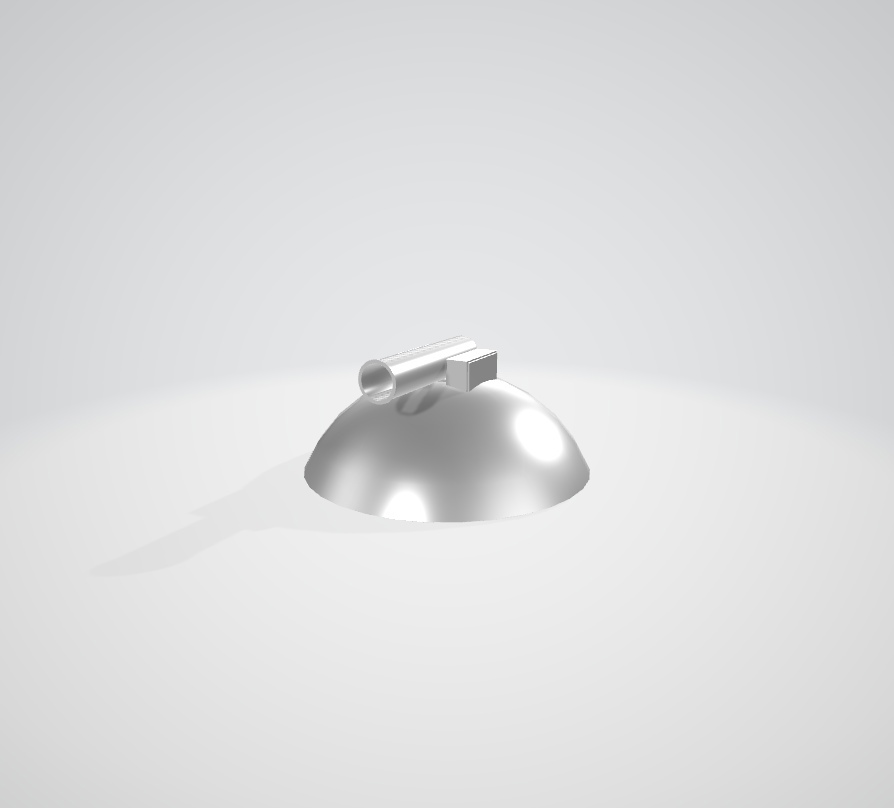
\includegraphics[scale=0.25]{images/5.jpg}
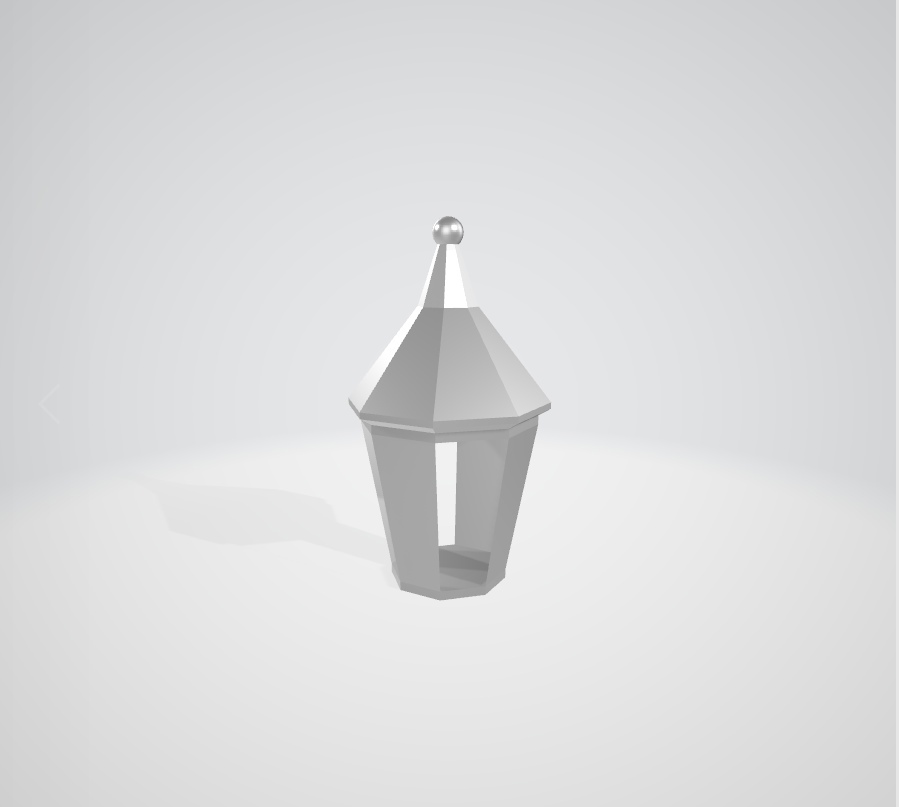
\includegraphics[scale=0.25]{images/6.jpg} \\
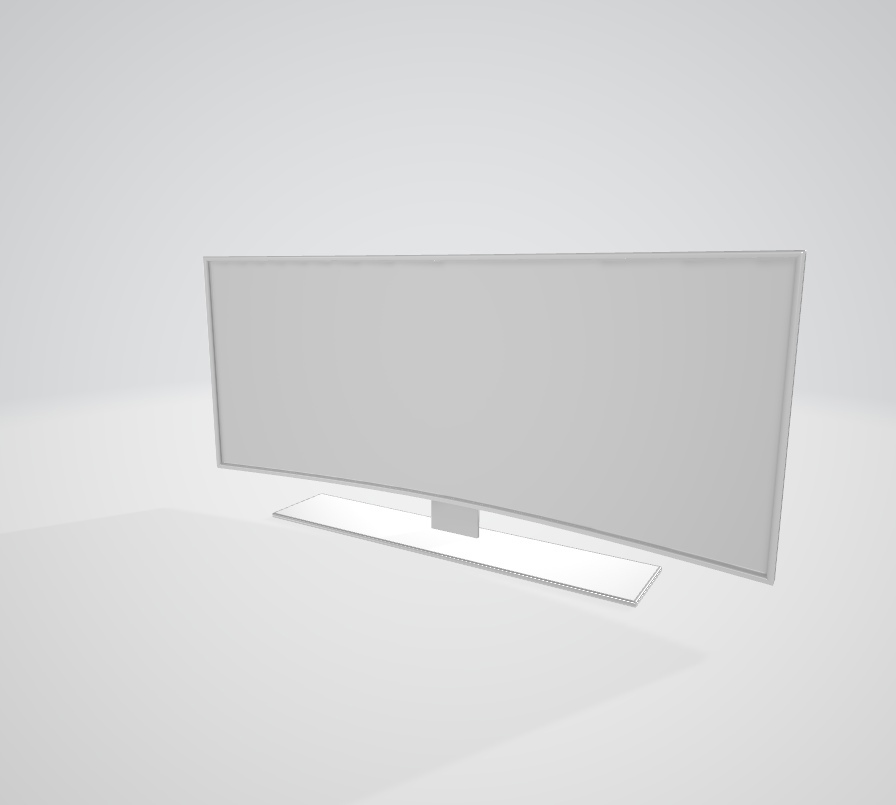
\includegraphics[scale=0.25]{images/7.jpg}
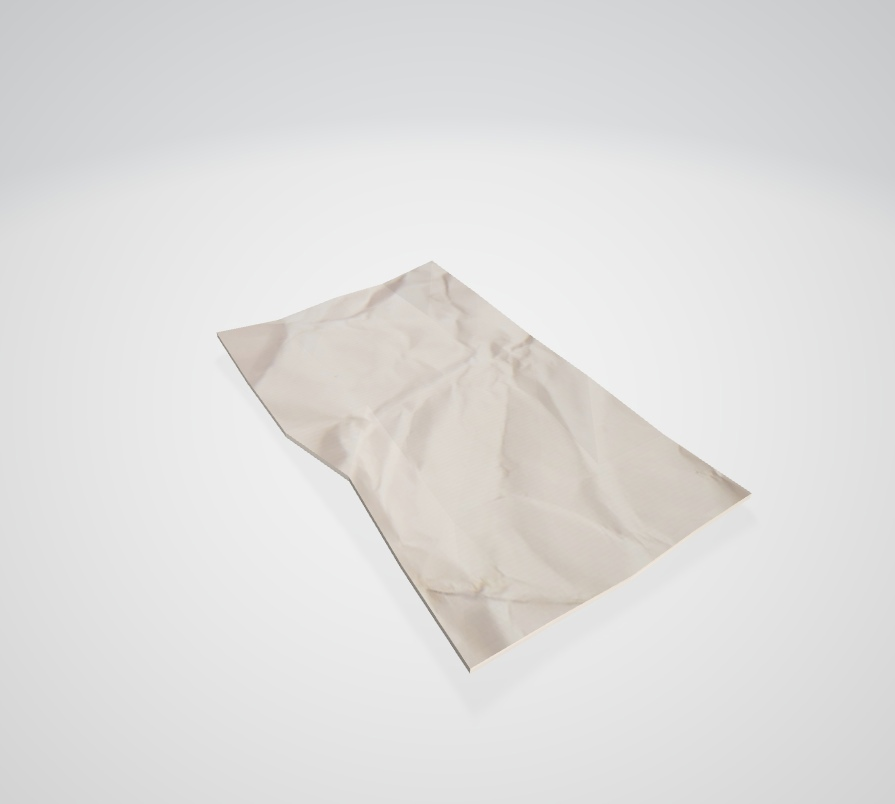
\includegraphics[scale=0.25]{images/8.jpg} \\
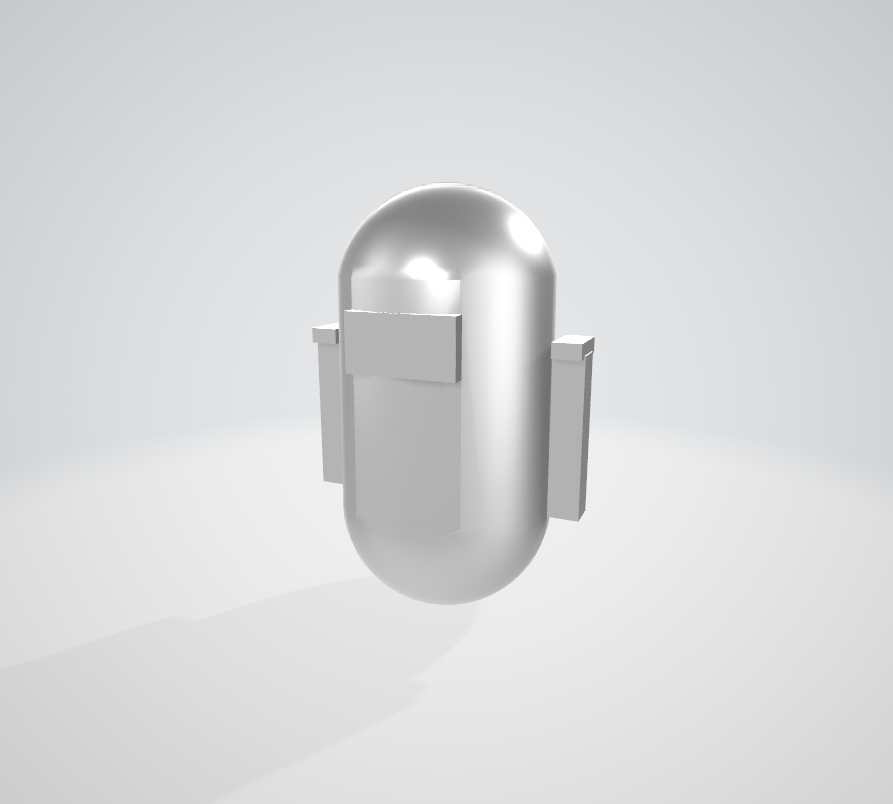
\includegraphics[scale=0.5]{images/9.jpg}

\pagebreak
\noindent {\bf Кадры из игры:}
\\
\noindent
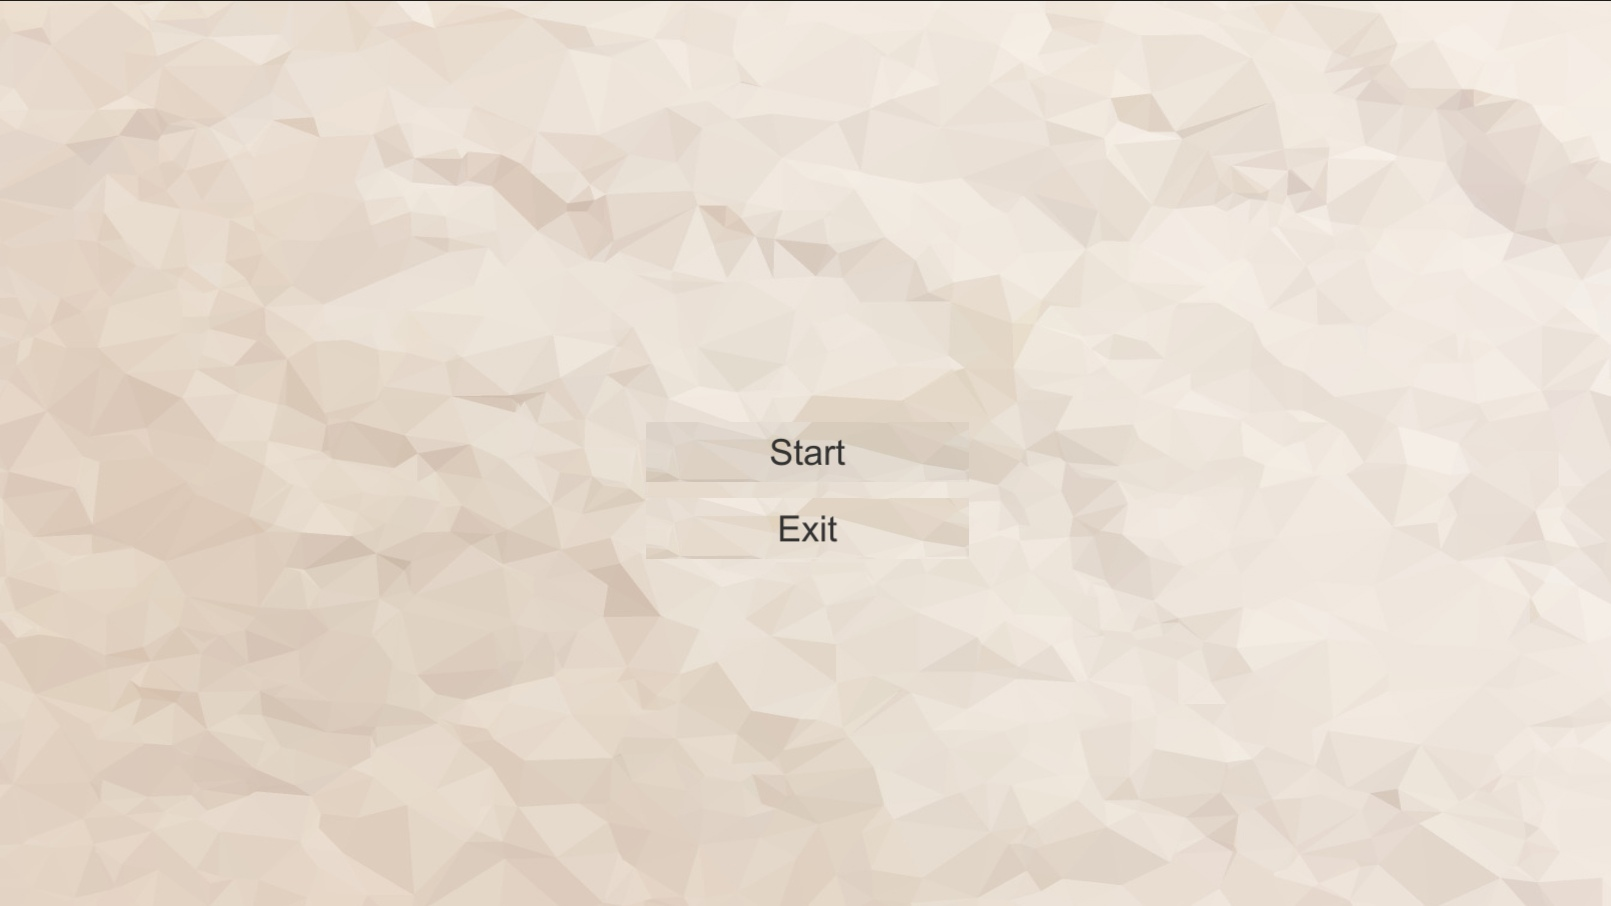
\includegraphics[scale=0.3]{images/21.jpg} \\
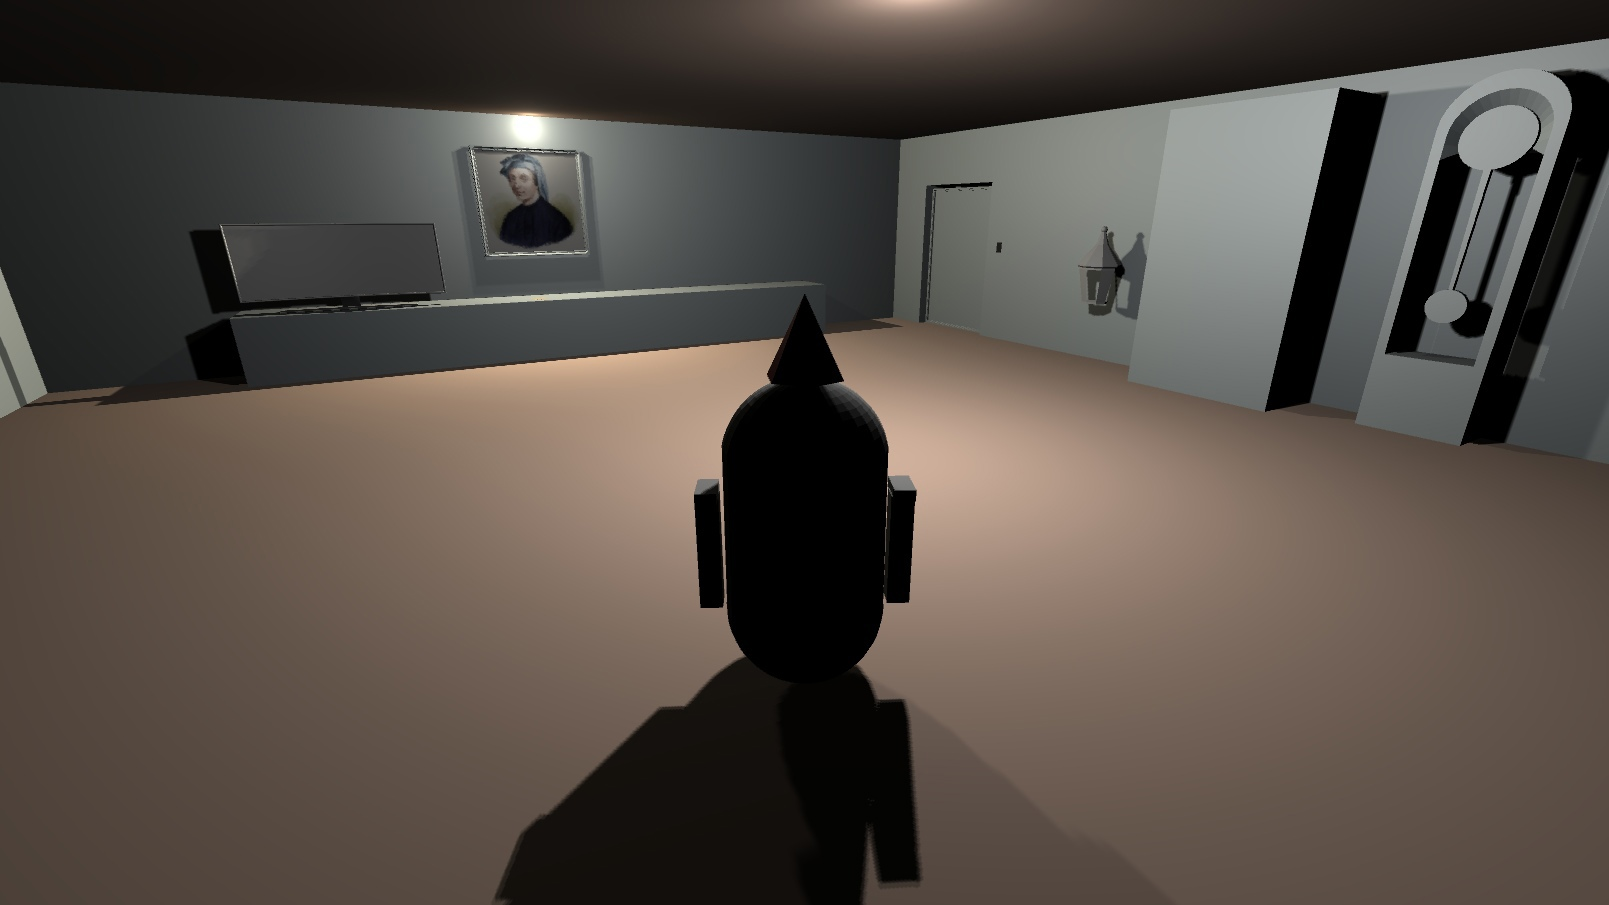
\includegraphics[scale=0.3]{images/22.jpg} \\
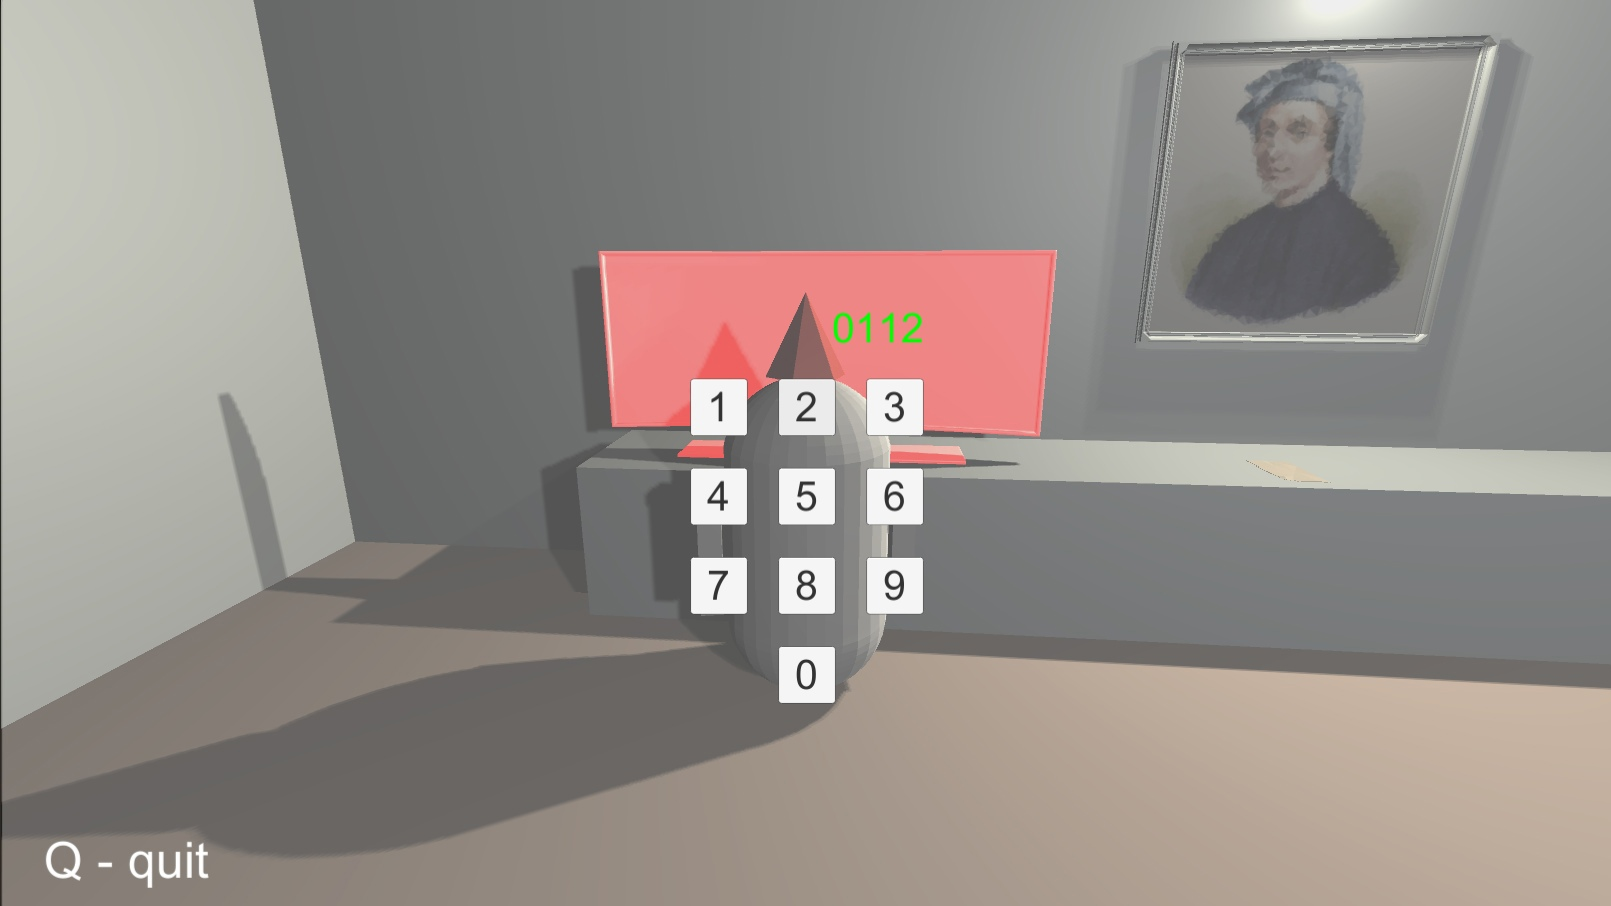
\includegraphics[scale=0.3]{images/23.jpg} \\
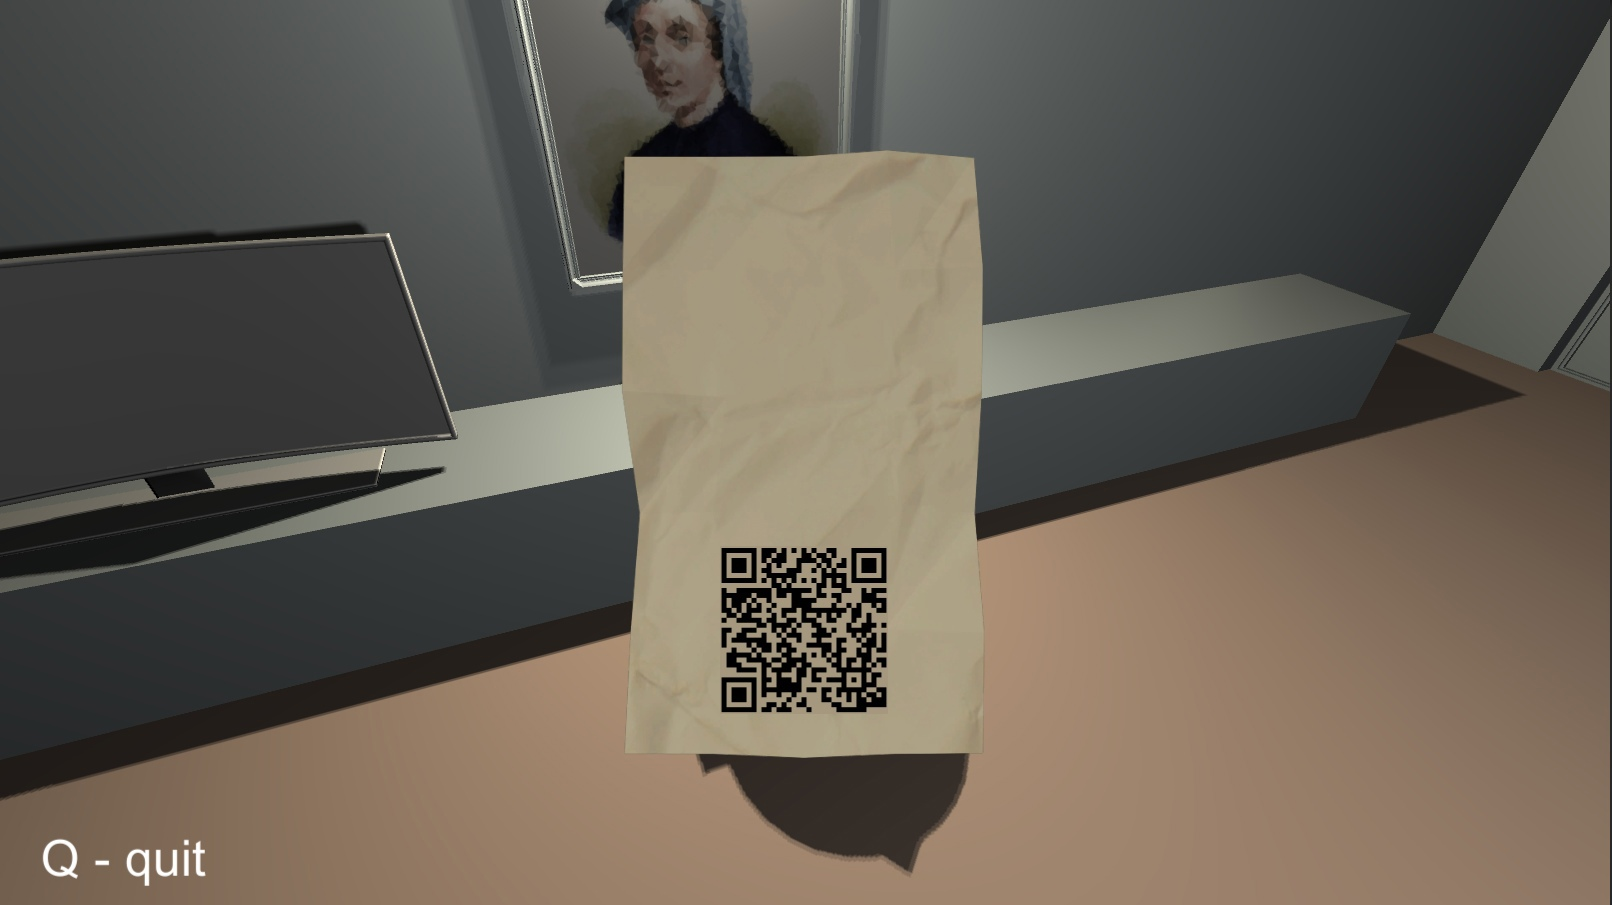
\includegraphics[scale=0.3]{images/24.jpg} \\
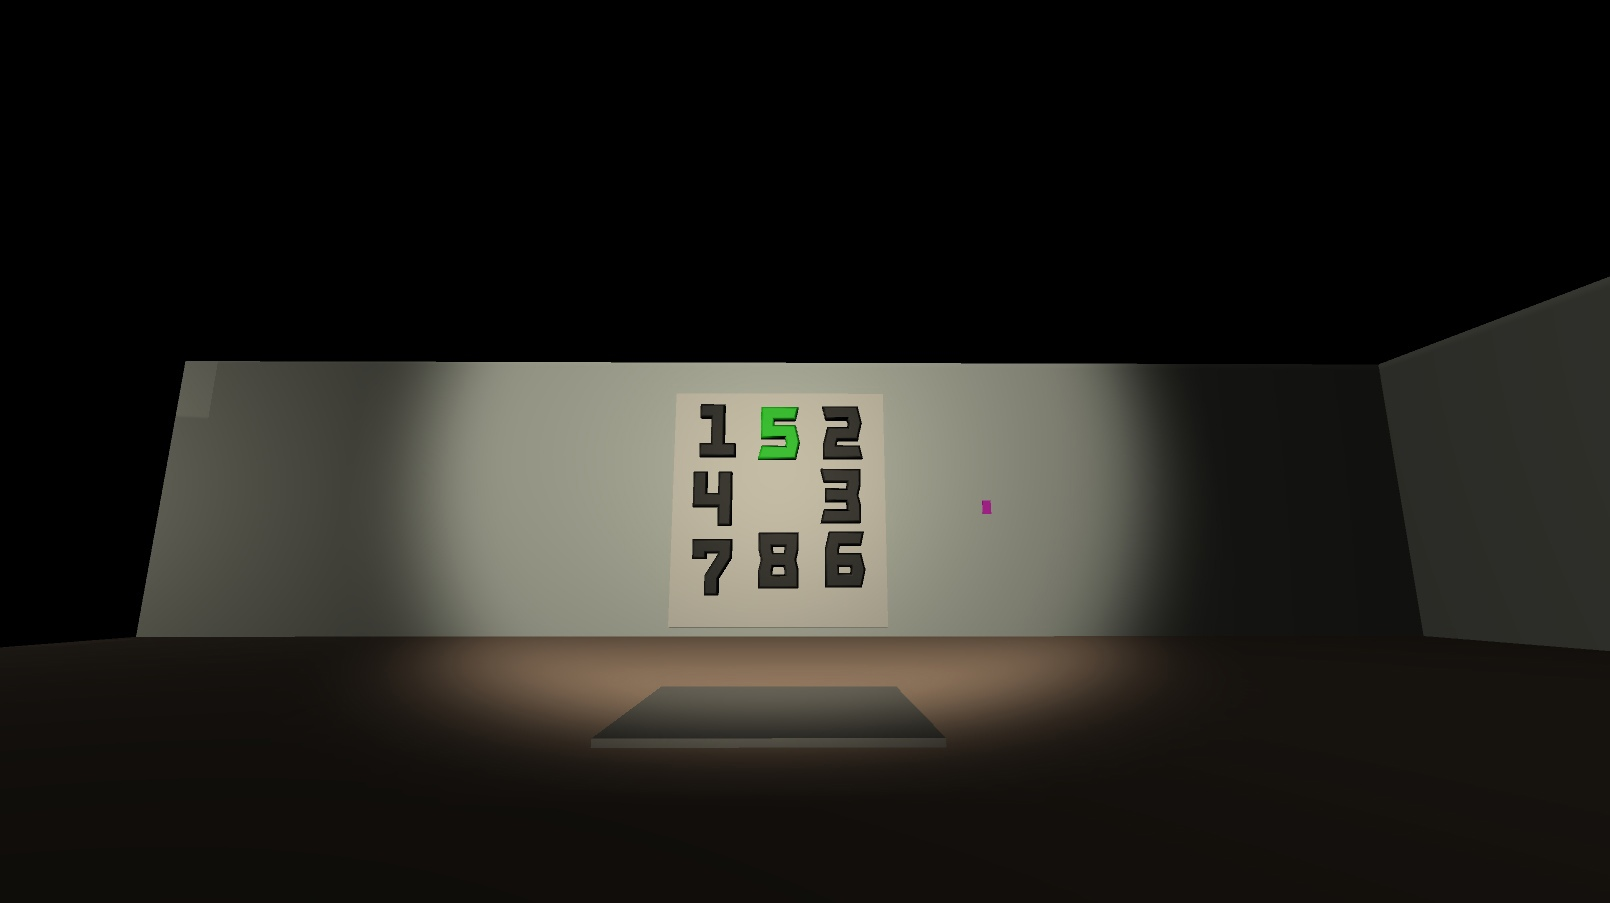
\includegraphics[scale=0.3]{images/25.jpg} \\
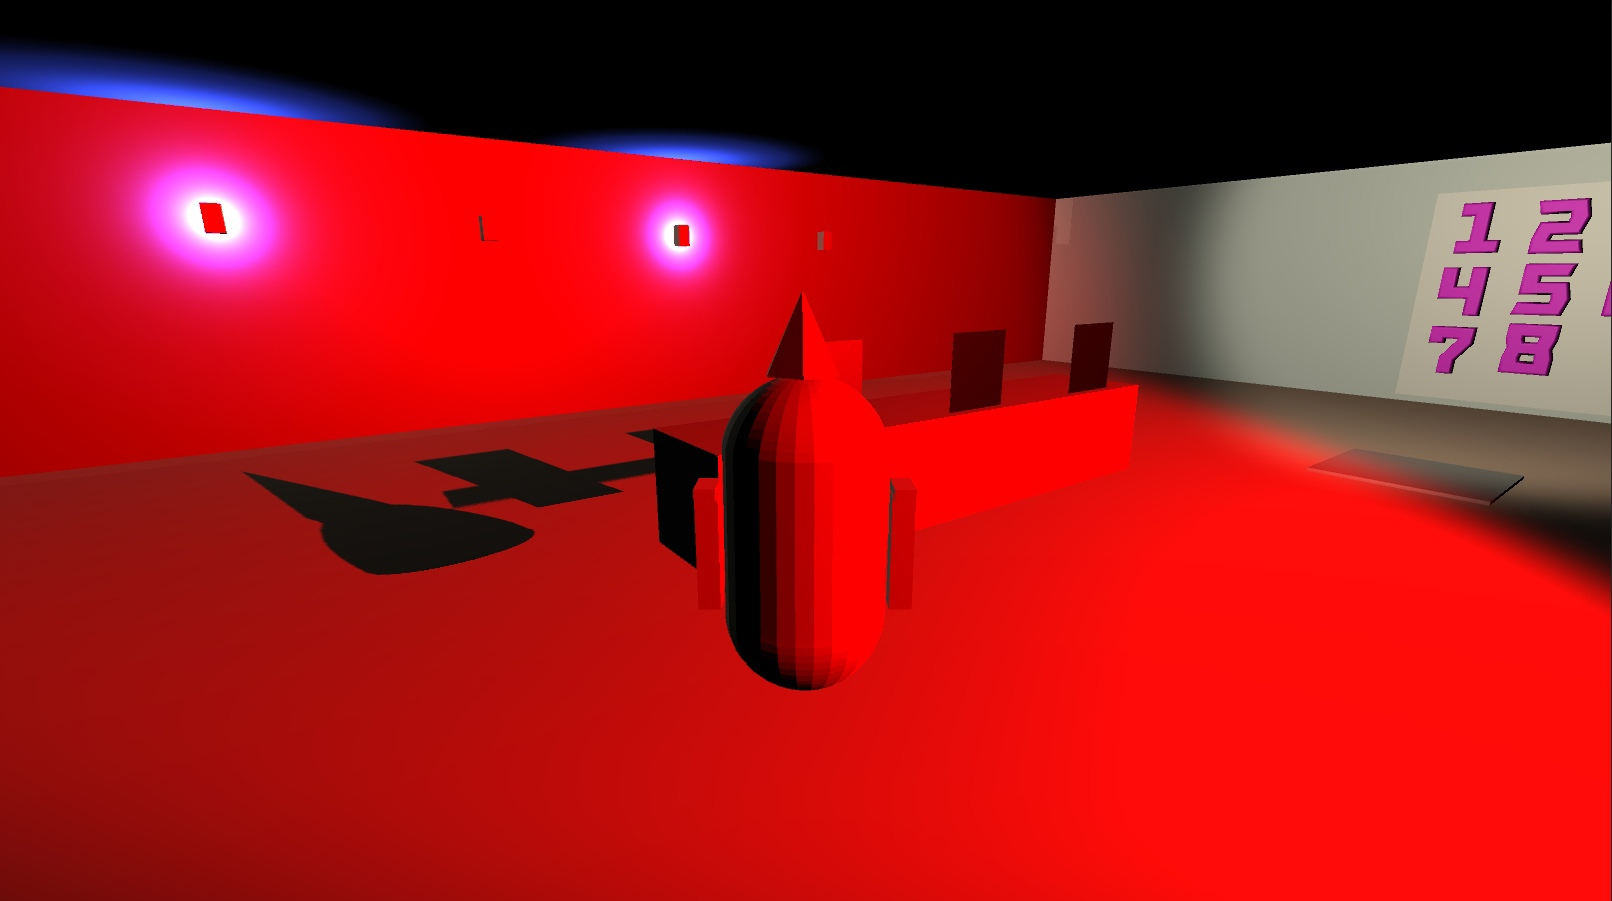
\includegraphics[scale=0.3]{images/26.jpg} \\
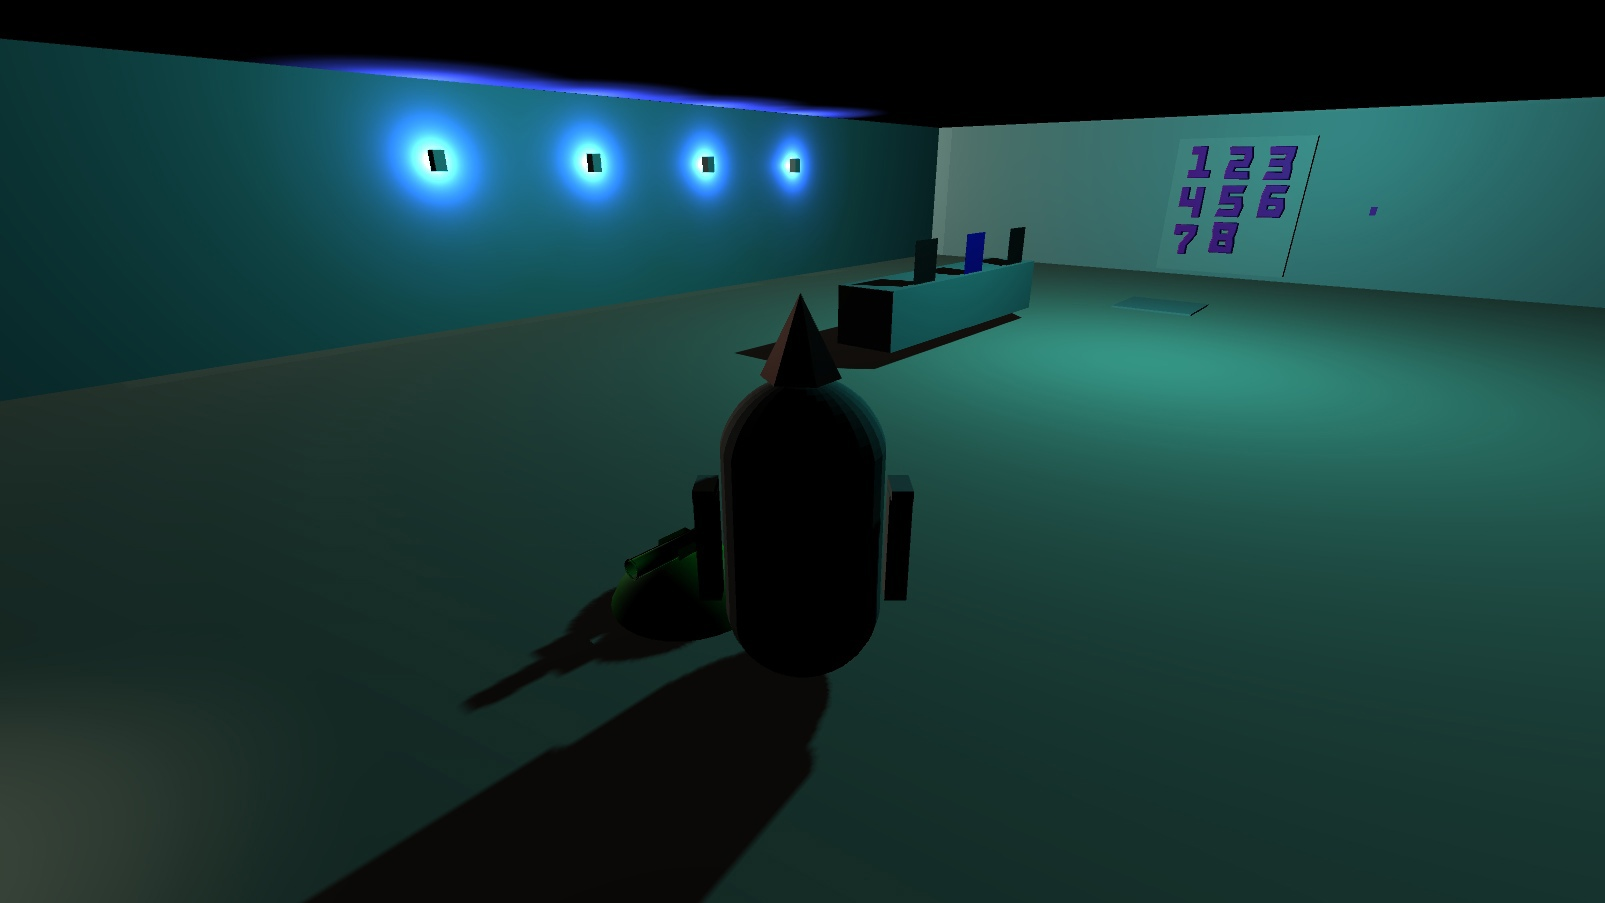
\includegraphics[scale=0.3]{images/27.jpg} \\
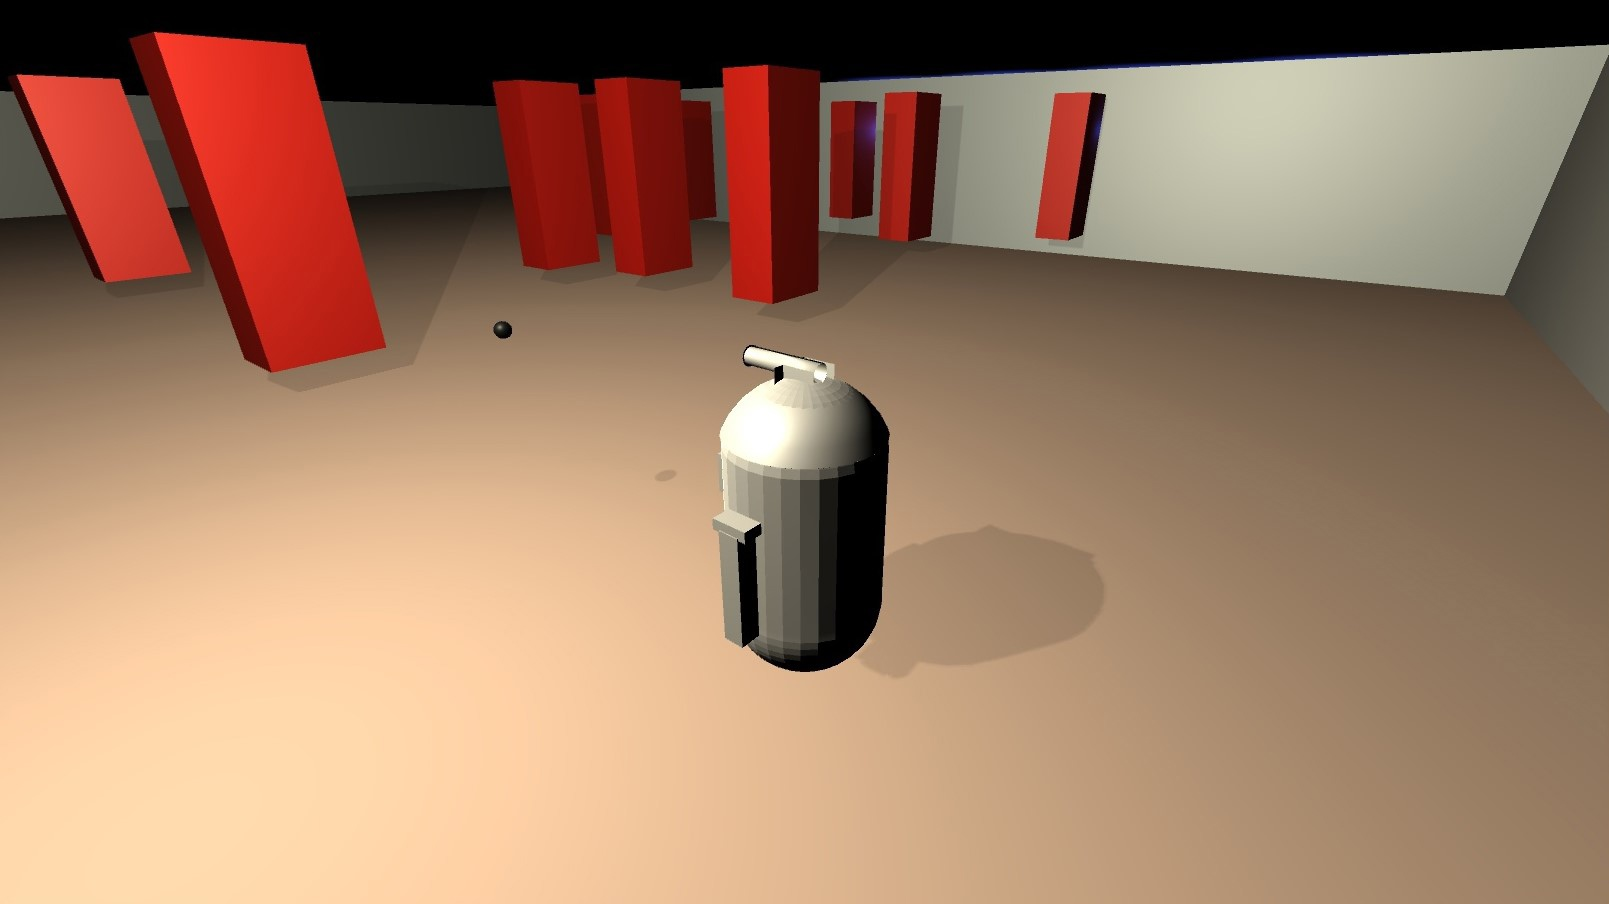
\includegraphics[scale=0.3]{images/28.jpg} \\

\section*{Тестирование}

\noindent {\bf Профайлер:}

На скриншотах показано, как большенство времени тратится на именно отрисовку объектов и просчет их физики, в то время как время работы скриптов составляет очень маленькую часть от всей времени отрисовки кадра. Средний фпс - 300 кадров в секунду.
\\
\noindent
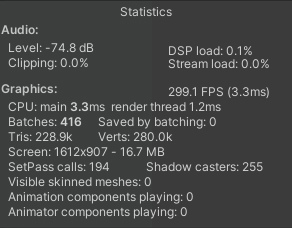
\includegraphics[scale=1]{images/11.jpg} \\
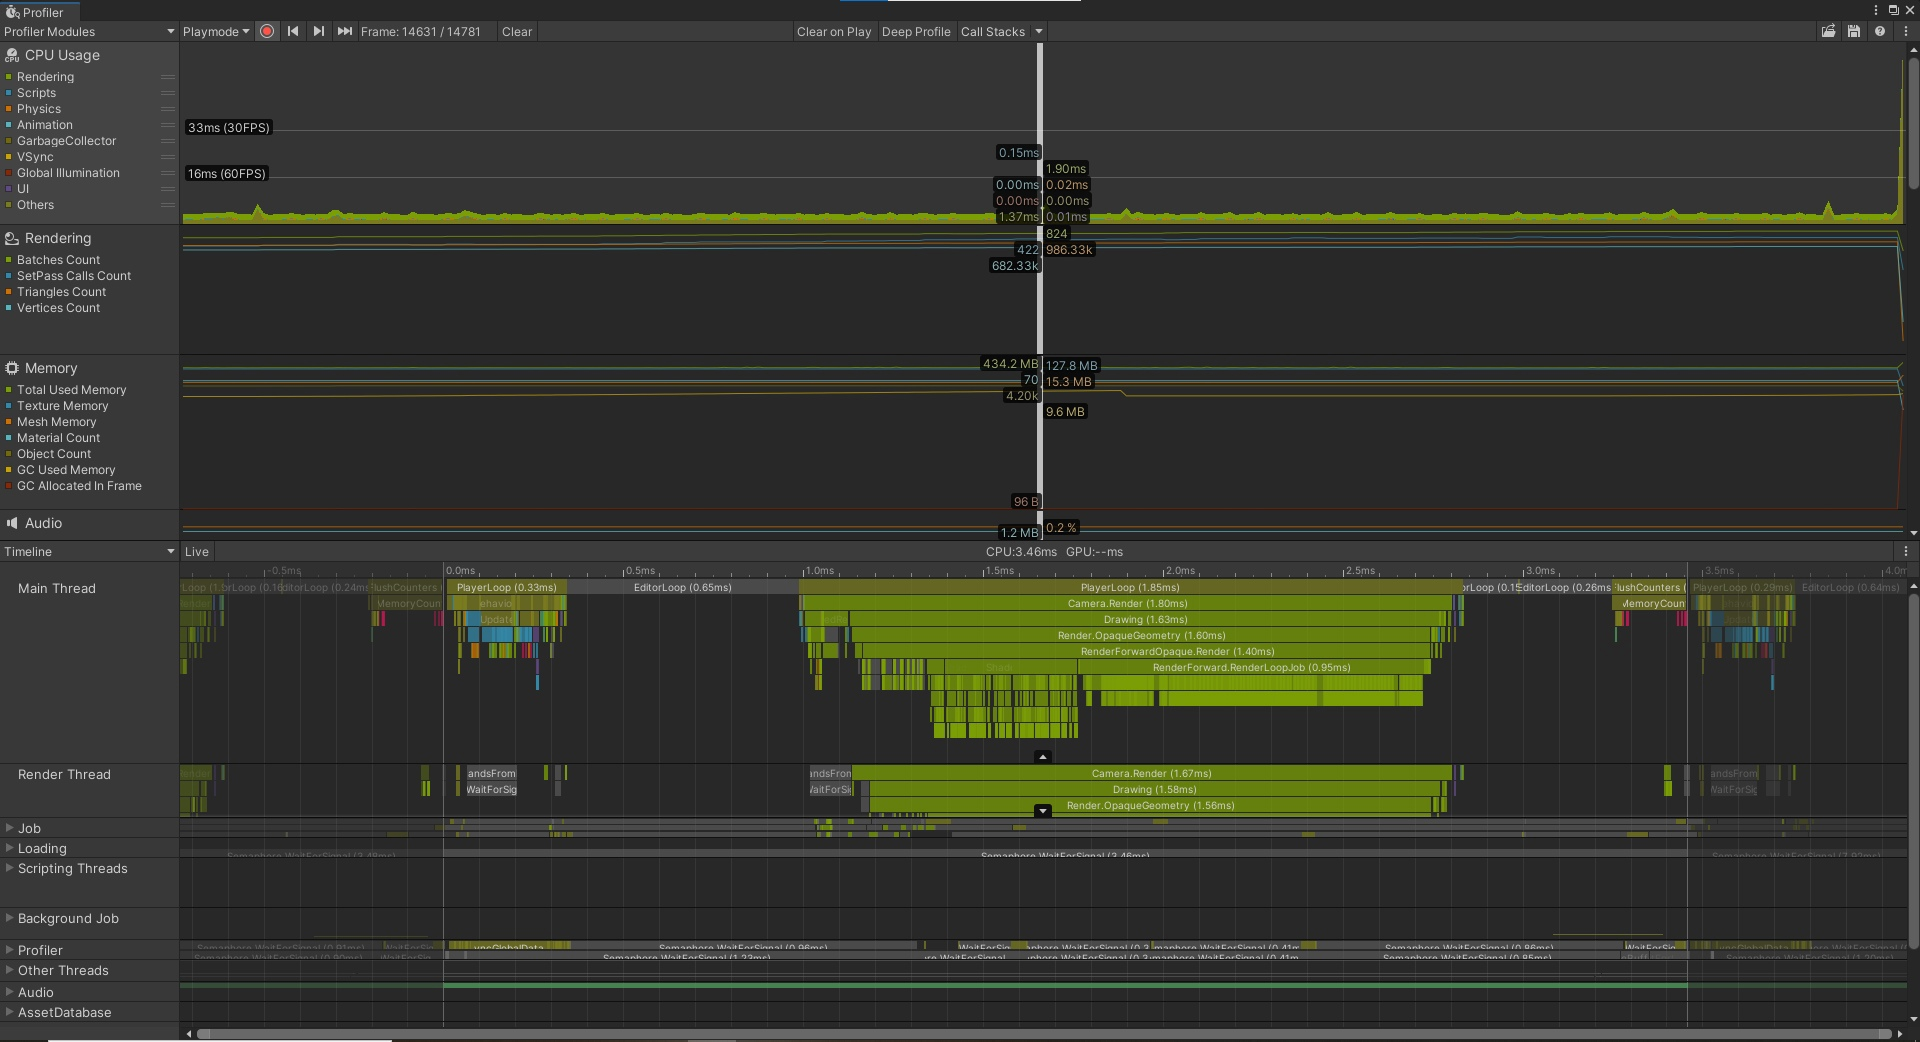
\includegraphics[scale=0.25]{images/12.jpg}

\section*{Ссылка на GitHub}

https://github.com/Igor743646/SummerPractise

\pagebreak
